\newcommand{\RequirementsTable}{%
\begin{table}[htbp]\small
\caption{Requirements traced to implementation and evidence. S: source inspected; E: backend or JVM executed; D: dated production-package checks on a phone; F: current isolated preview UI fixture on a phone.}\label{tab:requirements}
\begin{tabularx}{\textwidth}{@{}P{10mm}Y Y P{12mm}@{}}\toprule
ID & Requirement and component & Verification and scope & State\\\midrule
R1 & Older adult and caregiver views; MainActivity & Role selection, navigation and caregiver wearable guard checked on device & E/D/F\\
R2 & Reading storage and retrieval; readings API, SQLite & Idempotency, access and ordering tests pass & E\\
R3 & Tappable metric history; history API, MetricHistoryChartView & Mounted Day/Week/Month charts; weighted aggregation, gaps and consent tested & E/F\\
R4 & Three classes and confidence; ModelService, LearningActivity & Class, score and saved history in UI fixture; persistence and access tested separately & E/F\\
R5 & Stored alerts and review; alerts, private inbox & Sustained episode, recovery and independent caregiver review tested & E\\
R6 & Missing, invalid and disconnected states & Validation and relay policies tested; physical outage recovery outside this campaign & S/E\\
R7 & Roles, consent and credentials & Authentication, approved membership, TLS and revocation tested & E\\
R8 & Modular app and accessible navigation & JVM logic, tabs and enlarged registration checked; Activity coupling remains & E/D/F\\
R9 & Controlled development and contribution & Four main history commits establish repository-level development history & S\\
R10 & Synthetic demonstration and improvement & Isolated Learning insights; API episodes and matched backend comparison & E/F\\\bottomrule
\end{tabularx}
\end{table}}

\newcommand{\RoleTable}{%
\begin{table}[htbp]\small
\caption{Role behaviour in the current release. Server checks enforce access; the Android UI also restricts wearable controls to the older adult.}\label{tab:roles}
\begin{tabularx}{\textwidth}{@{}Y P{35mm}P{35mm}@{}}\toprule
Action & Older adult & Approved caregiver\\\midrule
Read current overview and alert history & Own account & Linked adults only\\
Submit own sensor snapshots & Own account & Cannot impersonate adult\\
Approve or revoke caregiver & Own circle & Cannot self approve\\
Review alert & View own history & Own acknowledgement only\\
Account and connection settings & After sign in & After sign in\\
Guided wearable connection & Own wearable only & Controls unavailable\\
Metric chart and period navigation & Own retained readings & Linked adult's readings\\
Synthetic AI class and confidence & Add and review own exercises & Review linked adult's exercises\\
Registration accessibility & 200\% layout checked & 200\% layout checked\\\bottomrule
\end{tabularx}
\end{table}}

\newcommand{\DatasetFigure}{%
\begin{figure}[htbp]\centering
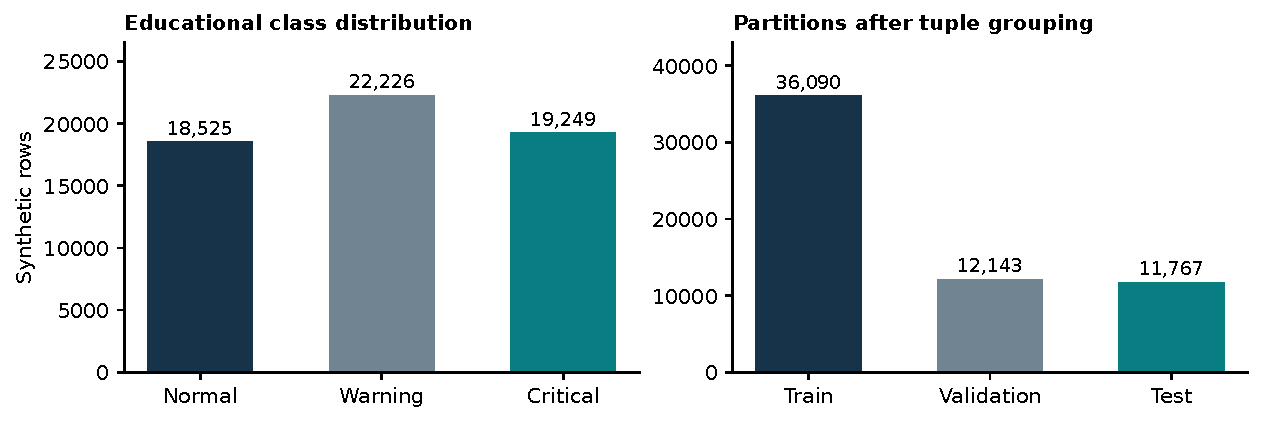
\includegraphics[width=0.95\textwidth]{dataset_summary.pdf}
\caption{Class balance and row partitions from the saved training metadata. Splitting operates on unique feature tuples, so row proportions differ slightly from 60/20/20. These labels are educational categories.}\label{fig:dataset}
\end{figure}}

\newcommand{\MetricsTable}{%
\begin{table}[htbp]\small\centering
\caption{Local validation and test performance. P, R and F1 are macro averages; all values are percentages. Validation selects the model.}\label{tab:metrics}
\begin{tabular}{@{}llrrrrr@{}}\toprule
Model & Partition & Accuracy & P & R & F1 & Critical R\\\midrule
Logistic regression & Validation & 75.15 & 75.18 & 75.53 & 75.34 & 73.85\\
Random Forest & Validation & 100.00 & 100.00 & 100.00 & 100.00 & 100.00\\\addlinespace
Logistic regression & Test & 75.35 & 75.85 & 76.46 & 76.11 & 76.54\\
Random Forest & Test & 100.00 & 100.00 & 100.00 & 100.00 & 100.00\\\bottomrule
\end{tabular}
\end{table}}

\newcommand{\ConfusionFigure}{%
\begin{figure}[htbp]\centering
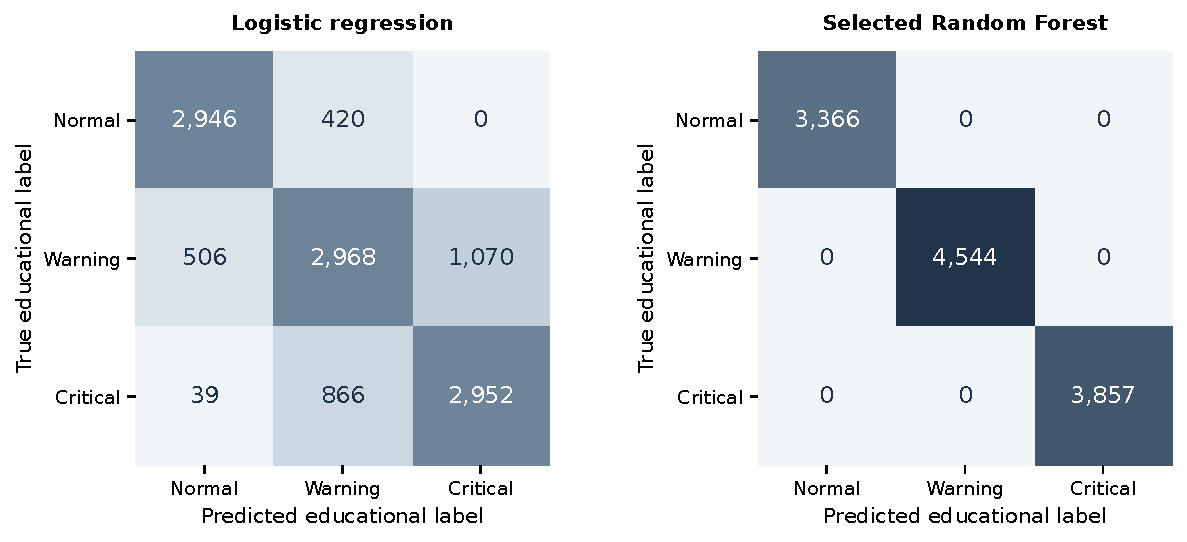
\includegraphics[width=\textwidth]{confusion_comparison.pdf}
\caption{Confusion matrices for 11,767 locally held out synthetic rows. The selected forest reconstructs the rule derived labels perfectly on this split. This is neither clinical validation nor an assessor hidden test.}\label{fig:confusion}
\end{figure}}

\newcommand{\RatesTable}{%
\begin{table}[htbp]\small
\caption{Classification errors and alert observations with explicit denominators. Classifier rates do not measure phone delivery failures.}\label{tab:rates}
\begin{tabularx}{\textwidth}{@{}Y P{32mm}P{31mm}@{}}\toprule
Measure and denominator & Logistic regression & Random Forest\\\midrule
Missed Critical classification: predicted other class / all true Critical & 905/3,857 = 23.46\% & 0/3,857 = 0\%\\
False Warning on Normal: predicted Warning / all true Normal & 420/3,366 = 12.48\% & 0/3,366 = 0\%\\
False Critical on noncritical: predicted Critical / true Normal or Warning & 1,070/7,910 = 13.53\% & 0/7,910 = 0\%\\\midrule
Server episode campaign & \multicolumn{2}{l}{20/20 created; 0/20 duplicate episodes}\\
Missed Critical alert at caregiver phone & \multicolumn{2}{l}{Outside server benchmark scope}\\
False Warning delivered to caregiver & \multicolumn{2}{l}{Outside server benchmark scope}\\\bottomrule
\end{tabularx}
\end{table}}

\newcommand{\VerificationTable}{%
\begin{table}[H]\small
\caption{Current revision and dated baseline verification. Counts are not added because the units and campaigns differ.}\label{tab:verification}
\begin{tabularx}{\textwidth}{@{}P{34mm}P{25mm}Y@{}}\toprule
Evidence & Result & Scope and exclusions\\\midrule
Current Python suite & \CurrentPythonResult & Current revision software record; units are tests\\
Current JVM suite & \CurrentJvmResult & Pure Java checks; not Android runtime acceptance\\
Metric history suite & \CurrentHistoryResult & Weighted means, validity, gaps, boundaries, retention and consent\\
Learning record suite & \CurrentLearningResult & Synthetic persistence, idempotency, authorisation and revocation\\
Current Android scope & Code \CurrentVersionCode & \CurrentAndroidResult\\
Current HTTPS scope & \CurrentIntegrationResult & Distinct from physical Bluetooth or caregiver delivery\\\midrule
Baseline Python/JVM & 88 / 2,830 & 26 October records: Python tests / JVM assertions\\
Baseline HTTPS & 17/17 checks & Loopback TLS, fictional accounts; no phone or Bluetooth\\
Baseline APK and UI & Code 13; 709 checks & Installed on Samsung SM-S948B, Android 17; registration at 200\% font scale. APK SHA-256 \texttt{417c12ef\ldots206378}\\
Baseline benchmark & 20/20 episodes & Temporary databases; no duplicate retry or sustained episodes\\\bottomrule
\end{tabularx}
\end{table}}

\newcommand{\TimingTable}{%
\begin{table}[H]\small
\caption{26 October baseline server processing measurements in milliseconds. Percentiles use linear interpolation; no transport or Android latency is included.}\label{tab:timing}
\begin{tabularx}{\textwidth}{@{}Y rrrr@{}}\toprule
Timed operation & N & Mean & p50 & p95\\\midrule
Warm authenticated classification & 25 & 17.34 & 16.85 & 19.87\\
Third qualifying reading and episode commit & 20 & 7.08 & 6.95 & 9.09\\
Third reading through authenticated inbox GET & 20 & 12.24 & 12.02 & 15.02\\
Cold classification including model load & 1 & 1,059.29 & --- & ---\\\bottomrule
\end{tabularx}
\smallskip\par\footnotesize The first two episode samples were already stored. Inbox timing uses the fictional adult's inbox; caregiver fanout is verified separately by the HTTPS integration fixture.
\end{table}}
